\section{DFS and BFS}

%%%%%%%%%%%%%%%
\begin{frame}{Classifying edges}
  \begin{definition}[Classifying edges]
    Given a dfs/bfs traversal:
    \begin{itemize}
      \item Tree edge
      \item Back edge
      \item Forward edge
      \item Cross edge
    \end{itemize}
  \end{definition}

  \begin{alertblock}{Remarks:}
    \begin{itemize}
      \item Applicable to both DFS and BFS
      \item With respect to DFS/BFS trees
    \end{itemize}
  \end{alertblock}
\end{frame}
%%%%%%%%%%%%%%%
\begin{frame}{Classifying edges \pno{3.4.1}}
  \begin{figure}
    \begin{subfigure}{0.50\linewidth}
      \centering
      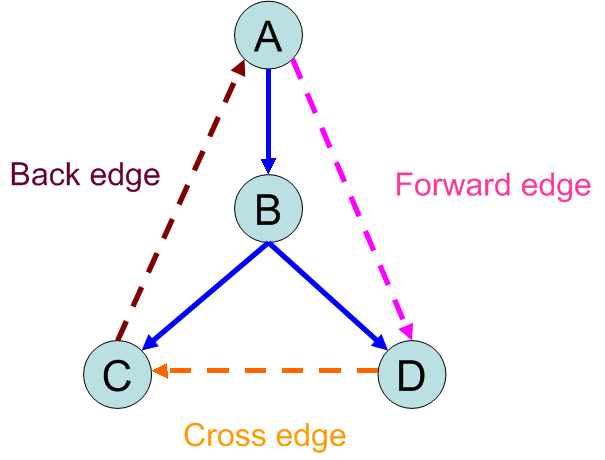
\includegraphics[width=0.50\textwidth]{figures/dfs-digraph.png}
      \caption{DFS on directed graph.}
    \end{subfigure}%
    \begin{subfigure}{0.50\linewidth}
      \centering
      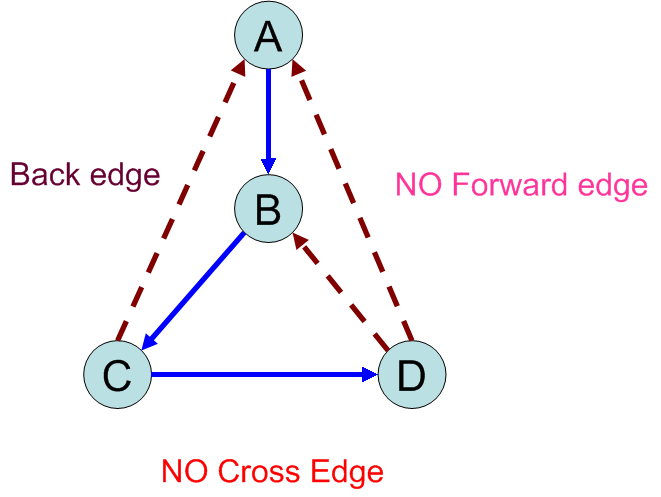
\includegraphics[width=0.50\textwidth]{figures/dfs-undirected.png}
      \caption{DFS on undirected graph.}
    \end{subfigure}

    \begin{subfigure}{0.50\linewidth}
      \centering
      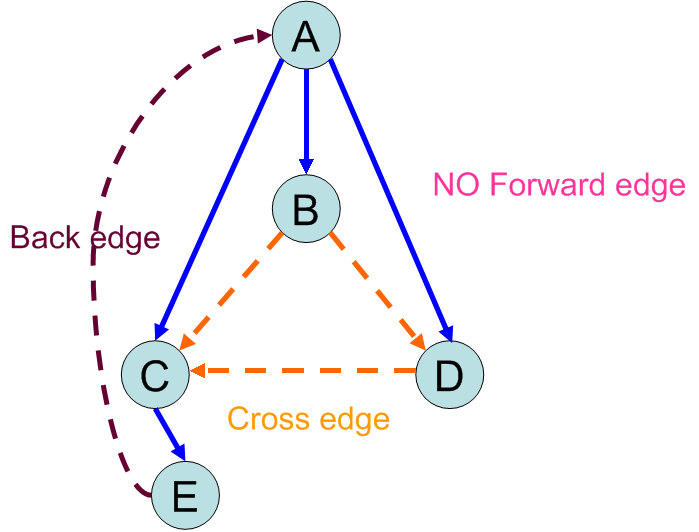
\includegraphics[width=0.50\textwidth]{figures/bfs-digraph.png}
      \caption{BFS on directed graph.}
    \end{subfigure}%
    \begin{subfigure}{0.50\linewidth}
      \centering
      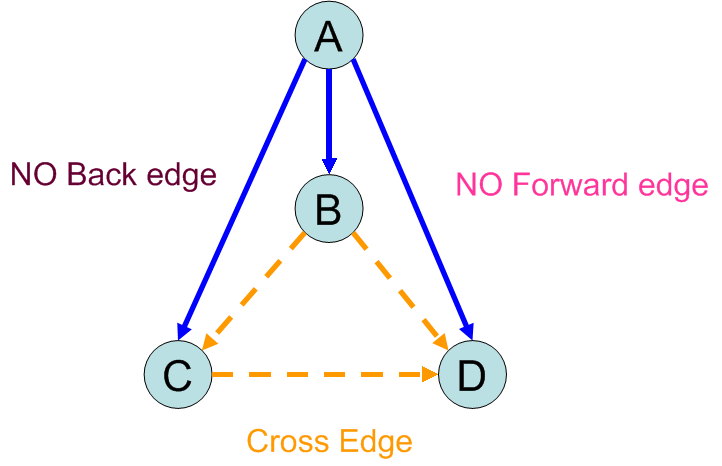
\includegraphics[width=0.60\textwidth]{figures/bfs-undirected.png}
      \caption{BFS on undirected graph.}
    \end{subfigure}
  \end{figure}
\end{frame}
%%%%%%%%%%%%%%%
\begin{frame}{Classifying edges}
  \begin{exampleblock}{DFS tree and BFS tree coincide \pno{3.4.30}}
    $G = (V,E), v \in V$. DFS tree $T$ = BFS tree $T'$.

    \begin{itemize}
      \item $G$ is an undirected graph $\Rightarrow$ $G = T$.
      \item $G$ is a digraph $\Rightarrow^{?}$ $G = T$.
    \end{itemize}
  \end{exampleblock}

  \begin{block}{Solution.}
    \begin{itemize}
      \item $T$: tree + back; $T'$: tree + cross
      \item $T$: tree + back + forward + cross; $T'$: tree + back + cross 
    \end{itemize}
  \end{block}
\end{frame}
%%%%%%%%%%%%%%%
\begin{frame}{Distance constraints for BFS}
  \begin{exampleblock}{Distance constraints for BFS \pno{3.4.4}}
    \begin{columns}[t]
      \column{0.40\textwidth}
        BFS on digraph:
	\begin{description}
	  \item[TE:] $d[v] = d[u] + 1$
	  \item[BE:] $0 \le d[v] \le d[u]$
	  \item[CE:] $d[v] \le d[u] + 1$
	\end{description}
      \column{0.60\textwidth}
        BFS on undirected graph:
	\begin{description}
	  \item[TE:] $d[v] = d[u] + 1$
	  \item[CE:] $d[v] = d[u] \lor d[v] = d[u] + 1$ 
	\end{description}
    \end{columns}
  \end{exampleblock}

  \begin{block}{Solution to ``\emph{CE} in BFS on \emph{undirected} graph''.}
    \begin{itemize}
      \item $d[v] = d[u], d[v] = d[u] + 1$
      \item $d[v] < d[u], d[v] > d[u] + 1$
    \end{itemize}
  \end{block}

  \begin{alertblock}{Remark.}
    \begin{itemize}
      \item BFS tree defines a \emph{shortest-path} from its root to every other node.
      \item Layers in BFS on \emph{undirected} graph $\Rightarrow$ bipartite testing \pno{3.4.26}
    \end{itemize}
  \end{alertblock}
\end{frame}
%%%%%%%%%%%%%%%
